\subsection{Visualizzazione di un elemento del diagramma di dispersione}

\begin{figure}[H]
    \centering
    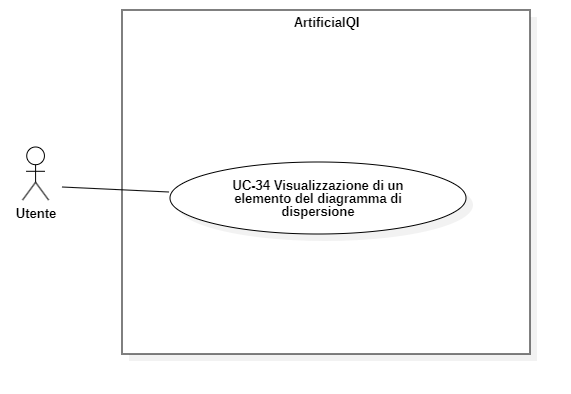
\includegraphics[scale=0.6]{Sezioni/UseCase/Immagini/InterazioneDiagrammaDispersione}
    \caption{Diagramma per la visualizzazione di un elemento del diagramma di dispersione.}
\end{figure}

\begin{usecase}{UC-37}{Visualizzazione di un elemento del diagramma di dispersione}
    \label{uc:UC-37}    
    
    \req{} 

    \pre{
        \item L'utente sta visualizzando i risultati del test caricato o sta visualizzando il confronto tra i singoli risultati di due test confrontati
    }

    \post{
        \item L'utente viene riportato al risultato relativo al risultato rappresentato dal punto del diagramma coinvolto nell'interazione 
    }
    
    \actor{Utente}

    \subactors{}

    \trigger{L'utente vuole visualizzare un elemento della pagina dei risultati del test}
    
    \inc{}

    \base{}

    \scenario{
        \item L'utente interagisce con un punto del diagramma di dispersione
        \item Il sistema rimanda l'utente al risultato che il punto rappresenta
    }

    \subscenario{}
\end{usecase}
